\section{Trace\textit{a} Metamodel}\label{sec:metamodel}
\begin{figure}[ht] 
	\centering
	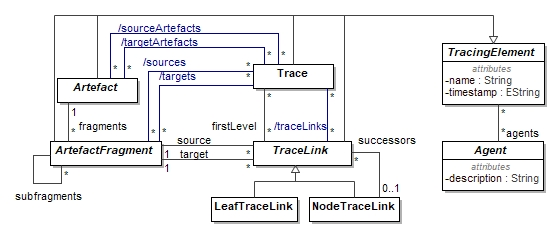
\includegraphics[width=.99\linewidth]{images/core.jpg}
	\caption{Core compositional nature of the Tracea}
	\label{fig:mm-core}
\end{figure}

Based on the previous analysis, we present in this section a new traceability metamodel, called Trace\textit{a}. We aim not to present yet another traceability metamodel but one that learns from and supersedes previous proposals in order to provide a more complete metamodel %\footnote{As any metamodel, OCL constraints \cite{CabotG12} could be used to define additional well-formedness rules.} 
 that also responds  to the requirements made explicit in Section \ref{sec:requirements}. 
%In the course of producing this metamodel, we have tried to be as objective and inclusive as possible. To this extend we use existing knowledge on adaptable traceability which we augment with quality aspects found missing in the literature of the field.
To foster legibility, we have added a simple but complete example of the use of our metamodel to conclude this section.

\subsection{Adaptable and configurable traces} 
 
%As we have seen, there exists many approaches addressing the issue of adaptability. 
In Trace\textit{a}, we start from the common core trace representation in several of the existing metamodels but expand and refine it with a more configurable structure that allows one to define the proper level of granularity. 

\subsubsection{Fine grain tracing structure.} The excerpt in Fig. \ref{fig:mm-core} describes the composition scheme of links into a forest-like structure. Its atomic elements are \texttt{TraceLinks}. A trace link refers to a source and a target \texttt{ArtefactFragment}(see below). It may be a leaf -- which means it has no successor links ; or a node -- which means the trace does not \textit{end} with this link. A \texttt{Tracelink} is a composite of \texttt{LeafTraceLink} and \texttt{LeafTraceNode}. A \texttt{Trace} starts from a set of trace links "\texttt{firstLevel}" that connect to their respective trees. The set of derived \texttt{TraceLinks} from the transitive closure of \texttt{firstLevel} is contained in the reference \texttt{traceLinks}. In the same manner, the set of source and target artefacts and fragments of traces (see blue references in Fig.~\ref{fig:mm-core}) is derived as well (see Listing \ref{lst:ocl}).  \texttt{Trace} and \texttt{TraceLink} are subtypes of \texttt{TracingElement} with a unique identifier (name), a timestamp to address consistency issues (see below), and one or more \texttt{Agent} related. 


\lstset{style=mystyleocl}
\noindent\begin{minipage}[t]{.45\textwidth}
\begin{lstlisting}[frame=tlrb]{Name}
context Trace inv firstLevels:
   self.traceLinks
   ->includesAll(self.firstLevels)
   
context Trace inv sources:
   self.firstLevels
   ->collect(source)
   ->includesAll(self.sources)
   
context Trace inv targets:
   self.tracelinks
   ->collect(target)
   ->includesAll(self.targets)
\end{lstlisting}
\end{minipage}\hfill
\begin{minipage}[t]{.45\textwidth}
\begin{lstlisting}[caption={OCL expressions},frame=tlrb,label=lst:ocl]{Name}
context Trace inv sourceArtefacts:
   self.firstLevels
   ->collect(source)
   ->includesAll(
      self.sourceArtefacts.fragments)
   
context Trace inv targetArtefacts:
   self.tracelinks
   ->collect(target)
   ->includesAll(
      self.targetArtefacts.fragments)
\end{lstlisting}

\end{minipage}

\subsubsection{Adaptable artefacts and relationships.}
Existing traceability works differ a lot in the \textit{kind} of artefacts they target. A unified ontology of traced artefacts has yet emerged but a common approach is to distinguish between the nature of artefacts. \textit{I.e.,} from \textit{text intensive} (\textit{e.g.,} requirements, certification) to \textit{structure intensive} (\textit{e.g.,} source code, test cases).  
In Trace\textit{a}, we specialize \texttt{Artefact} with \texttt{TextArtefact}, \texttt{ModelArtefact}, \texttt{CodeArtefact}, and \texttt{TestArtefact}. 
The list is not exhaustive. These high-level types support the user in defining her own (sub)types. They are anchors to refine artefacts and their fragments at an adequate level of granularity.  

To freely adjust the granularity of the artefacts under scrutiny, Trace\textit{a} suggests the fragmentation of \texttt{Artefact}. An \texttt{ArtefactFragment} defines a part of an artefact that is of interest (\textit{e.g.,} a method in a class; a section in a text document). 
Trace\textit{a} implements a high-level separation for artefacts and relationships. This enables the separate customization of artefact types and the semantic relationships among them. The typing of relationships is versatile and we distinguish two kinds depending on the domain they apply to: \texttt{DomainType} and \texttt{EngineeringType}. In the former, the semantic of the final user (\textit{i.e.,} its domain of application) is targeted. In the latter, the concepts used by engineers or modelers are targeted (the domain of engineering). Same as for the artefact types, relationship types are also expected to be customized \cite{Olive02} when needed.

\Fig{fig:customization} shows an excerpt of the Trace\textit{a} metamodel that focus on aspects related to the adaptability of our approach.
\begin{figure}[ht]   
	\centering  
		\vspace{-0.4truecm}

	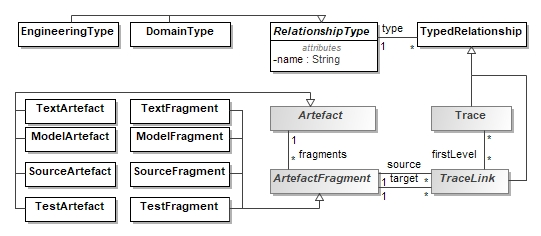
\includegraphics[width=.9\linewidth]{images/customization.jpg}
	\caption{Customization of artefacts and relationships in Tracea}
	\label{fig:customization}
\end{figure}

	\vspace{-0.4truecm}
\subsection{Confidence of trace links}
\begin{figure}[h] 
	\centering
		\vspace{-0.4truecm}

	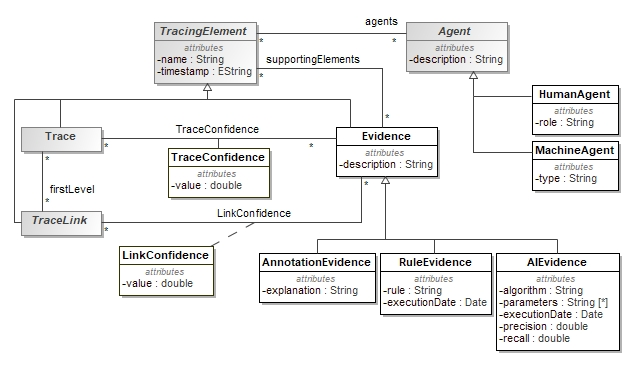
\includegraphics[width=.99\linewidth]{images/explainability.jpg}
	\caption{Representing Explaining traceability with confidence value, agents and evidences}
	\label{fig:explainability}
\end{figure}


In Trace\textit{a}, the confidence of a trace (\texttt{TraceConfidence}) or of a trace link (\texttt{Link- Confidence}) is a statement with a real number value representing the level (from 0 to 1) at which the trace is certain to exist in the system.
It is a statement about the relevance of a trace. A trace and its links are made by \texttt{Agents}. As illustrated in Fig.~\ref{fig:explainability}, an agent may be human (\textit{e.g.,} when traces are elicited manually), or an agent may be a machine (\textit{e.g.,} when an algorithm identify the trace automatically).


\subsection{Trace Consistency}
%\ugh{timestamp: every point knows if it complies with elements. Date comparison. update confidence with finer grain data to consider the decay of tracing artefacts.}
To address the issue of gradual decay, tracing elements must be considered alike with other software artefacts. Their evolution must be scrupulously and synchronously monitored. To be able to represent (and later reason) on the potential decay, we add a timestamp attribute to \texttt{TracingElement} (see Figure \ref{fig:explainability}), \textit{de facto} transforming all metaclasses inheriting from it in temporal elements. We can then use these timestamps to compare the age of a trace compared to the age of the elements traced by it and, if needed, update the confidence we have in that trace, or trace link, accordingly.

%This attribute is not sufficient by itself but assists the integration of tracing elements into version control systems (\textit{e.g.,} Git, SVN), or temporal management system such as TempoEMF.

\subsection{Explainability}
Traces are a key element in many software engineering activities. Therefore, engineers may not want to just take them at \textit{face value} but ask for explanations on how and when the trace was created. Previous subsection covered the \textit{when}, here we focus on the \textit{how}.

The degree of confidence may be justified with evidences, if they exist, to explain the rationale behind the quantitative value. In case of links automatically identified, an evidence instance can record the information necessary to reproduce the identification process or at least to partially explain it. 

More precisely, as can be seen in Fig. \ref{fig:explainability}, an evidence refines into three sub-types: \texttt{AnnotationEvidence} contains a textual description ; \texttt{RuleEvidence} contains a rule (or a set of rules) in a textual field, as well as the execution date ; and \texttt{AIEvidence} contains attributes that will help reproduce the learning scenario, \textit{e.g.,} the kind of algorithm, a reference to the training set and the associated precision and recall the algorithm, and others parameters. An \texttt{Evidence} explanation can also point to other supporting tracing elements. These elements testify, or illustrate the evidence and will be useful for later consistency check.

Every evidence is also optionally endorsed by a set of Human or Machine agents, which further helps in the explainability of the trace beyond the description and attribute values stored in the Evidence object itself.

\subsection{Illustrative example}


In this section, we introduce a simple illustrative example: tracing the impact of a change in the requirements onto their implementation in Java classes. We show through this example the customization of artefacts and relationships, the importance of a quality evaluation, and how we circumvent consequences of using AI-enabled modules for trace identification.
In this example, links are relating requirements to Java classes that undergo modifications. 

 
\subsubsection{Customization of artefacts and relationships}
In this case, a trace aligns two kinds of artefacts: 
\footnotesize\verb" Requirement specification " and \verb" Source class".
\normalsize

These artefacts are too complex to be used at a coarse level of granularity. Java classes may comprise hundreds (or even thousands) of lines of code, requirement specification documents contain hundreds of sections. To address this size issue, a source \texttt{Artefact} (e.g., a class) is decomposed into smaller part (such as methods). In the same manner, specification documents are decomposed into sections. Listing \ref{lst:declare} shows an excerpt of our textual concrete syntax applied to this example where we can see the fragmentation of artefacts. The structure of the traced system is first described with artefacts and fragments sections. For legibility concern, the only kind of relationship in that example is \texttt{Implement}, \textit{i.e.,} a source class \textit{implements} a requirement section. 


\lstset{style=mystyle}
\noindent\begin{minipage}[t]{.45\textwidth}
\begin{lstlisting}[caption={Artefacts, Fragments, Relationships, and Agents declaration},frame=tlrb,label=lst:declare]{Name}
artefacts {
   Requirement r_01 {fragments {sAuth, sLogout}},
   Source Login.java {fragments { mLogin, mLogError, mLogout }},
}
fragments {
   RequirementSection sAuth { },
   RequirementSection sLogout { },
   Method mLogin { },
   Method mLogError { },
   Method mLogOut { },
}
relationshiptypes {
   EngineeringType Implements {},
}
agents {
   HumanAgent 5e8a5T1e4,
   MachineAgent Rd15OUA5RD 
}
\end{lstlisting}
\end{minipage}\hfill
\begin{minipage}[t]{.45\textwidth}
\begin{lstlisting}[caption={Trace instance},frame=tlrb,label=lst:trace]{Name}
Trace ChangeImpact {
   tracelinks {  
      NodeTraceLink link01 { 
         source sAuth
         target mLogin
         successors {link02}
         relationshiptype Implements  
         agents 5e8a5T1e4
      },
      LeafTraceLink link02 { 
         source mLogin
         target mLogError
         relationshiptype Implements  
      },
      LeafTraceLink link03 { 
         source sLogout
         target mLogout
         successors {}
         relationshiptype Implements  
         agents Rd15OUA5RD
         confidence c01
      },
   }
}
\end{lstlisting}
\end{minipage}



The concrete traces are recorded as illustrated in Listing \ref{lst:trace}. A Trace is identifiable by its name and contains trace links whose composition is described through successors. This example is the minimalist expression of a trace. Each and every element is susceptible to refer to an \texttt{Agent} that indicates who and what is the nature of that “who” responsible for the edification of the trace. In our case, \texttt{link\_01} and \texttt{link\_03} have referees.

\subsubsection{Explainability for AI-enabled traceability}
There exists automated evaluation techniques for change impact that predicts which classes are most likely to change. In this scenario, a change in the requirements links to \textit{potentially} impacted classes, and to \textit{actually} modified classes. This distinction shows a distinction in nature of the links themselves. The former is more inclined to suffer a low level of confidence than the automatized latter. In our case, Listing \ref{lst:trace} shows that links \texttt{link\_01} and \texttt{link\_02} have been manually identified, and thus, there the confidence is \texttt{1.0} whereas \texttt{Link\_03} has been automatically suggested and boasts a confidence of \texttt{0.8}.
This level of confidence relies on evidence based on the algorithm employed, its parameterization, and its training setting. As can be seen in Listing \ref{lst:integrity}, a confidence is related to a \texttt{Trace} or a \texttt{TraceLink} and a set of \texttt{Evidence}s. %This representation simplifies the sections in which artefacts, fragments and links are defined. 

Evidences may be an \texttt{AIEvidence} like the one we just described, or \texttt{RuleEvide- nce} that relates patterns used for automatic identification, or \texttt{AnnotationEvidence} that simply contains a textual explanation of the evidence. 
In the example in Listing \ref{lst:integrity}, the confidence \texttt{value} represents the confidence in the prediction that the method \textit{mLogin} is impacted by a change in requirement \texttt{sAuth}. This prediction has been made using a specific algorithm which run settings can be found in the evidences section.

\begin{center}
\noindent\begin{minipage}[t]{.72\textwidth}
\begin{lstlisting}[caption={Confidence, evidence, and agency},frame=tlrb,label=lst:integrity]
confidences {
   Confidence c01 { 
      value 0.8
      evidence {Evidence_link03}
   },
}
evidences {
   AIEvidence Evidence_link03 {
      algorithmUsed "AI4All"
      parameters {"platform:/resource/training/pos_202012"}
      executionDate "20201207-123536"
      trainingResults .8 .7    
      impactedElements ("link02", mLogin, otherMethod) 
   },
}
agency {
   Rd15OUA5RD {Evidence_link03}
}
\end{lstlisting}
\end{minipage}
\end{center}


